\chapter[DATA WAREHOUSE COMO APOIO À ATIVIDADES DE MEDIÇÃO]{DATA WAREHOUSE COMO APOIO À ATIVIDADES DE MEDIÇÃO}
%\addcontentsline{toc}{chapter}{Introdução}
Pessoas que não conhecem o conceito de um \textit{Data Warehouse} muitas vezes se confundem com a real necessidade e finalidade de um banco de dados especializado para apoiar decisões. Na perspectiva do usuário, é útil saber\cite{pentaho2009}:
\begin{itemize}
\item Todas as informações estão em um mesmo lugar -  não há a necessidade de buscar informações em diversas fontes ou em estruturas de pastas confusas e infinitas; \cite{pentaho2009}
\item Informações atualizadas – as informações no \textit{Data Warehouse} são automaticamente carregadas e atualizadas em uma base regular; \cite{pentaho2009}
\item Acesso rápido – O \textit{Data Warehouse} é otimizado para a recuperação rápida de informação; \cite{pentaho2009}
\item Não há limites de tamanho - Um \textit{Data Warehouse} pode armazenar uma quantidade quase ilimitada de dados; \cite{pentaho2009}
\item Todo o histórico disponível – um \textit{Data Warehouse} mantém dados atuais e dados históricos de toda a informação. Isto significa que qualquer análise de tendências ou comparação ao longo do tempo é apoiado pelo \textit{Data Warehouse}. O histórico disponível não é apenas um conjunto de “dados antigos”, e sim um conjunto que agrega valor quando mudanças são controladas; \cite{pentaho2009}
\item Fácil de entender - O \textit{Data Warehouse} é modelado em termos de negócios e reflete a maneira como o stakeholder olha para a sua organização; \cite{pentaho2009}
\item Definições claras e uniformes – todo mundo na organização utiliza as mesmas definições, o que simplifica muito a comunicação; \cite{pentaho2009}
\item Dados padronizados – todos os dados estão em conformidade com as normas, o que significa que existe apenas uma definição e apenas um conjunto de valores para cada pedaço de informação; \cite{pentaho2009}
\end{itemize}

Quanto mais as informações de negócio são compartilhadas entre os projetos da organização, mais abrangente e eficaz é a capacidade da organização para avaliar os seus projetos. \cite{ spdw} \cite{kimball} afirma que a solução para o maior grau de integração e de normalização destas informações é representa-las com o uso de um Data Warehousing, onde as métricas são estruturadas de acordo com um modelo multidimensional.
Um \textit{Data Warehouse} (DW) é uma coleção de dados históricos integrados, não-voláteis, orientado a assunto, destinado a apoiar os processos de tomada de decisão durante um período específico de tempo. \cite{kimball}
\begin{itemize}
\item Integrado: Múltiplas fontes de dados que devem ser limpas, tratadas, convertidas, formatadas, e resumidas antes de serem armazenadas. \cite{kimball}
\item Orientado a assunto: organiza os dados pelos principais elementos do negócio para que os dados sejam analisados filtrando dados relevantes e excluindo os não úteis para a tomada de decisão. \cite{kimball}
\item Não-volátil: No DW, os dados são carregados e acessados, mas as atualizações geralmente ocorrem no ambiente operacional. \cite{kimball}
\item Variante no tempo: possibilita a manutenção de uma perspectiva histórica dos dados. \cite{kimball}
\end{itemize}

Um \textit{Data Warehouse} tem como objetivos 1) fornecer um fácil acesso às informações da organização; 2) apresentar consistentemente as informações da organização; 3) ser adaptativo e resistência a mudanças; 4) ser um ambiente seguro para proteger as informações da organização; 5) servir de base para a melhoria na tomada de decisões; e, 6) ser aceito pela comunidade de negócio.

\section{Componentes de um DW}

\begin{figure}[!htb]
	\centering
		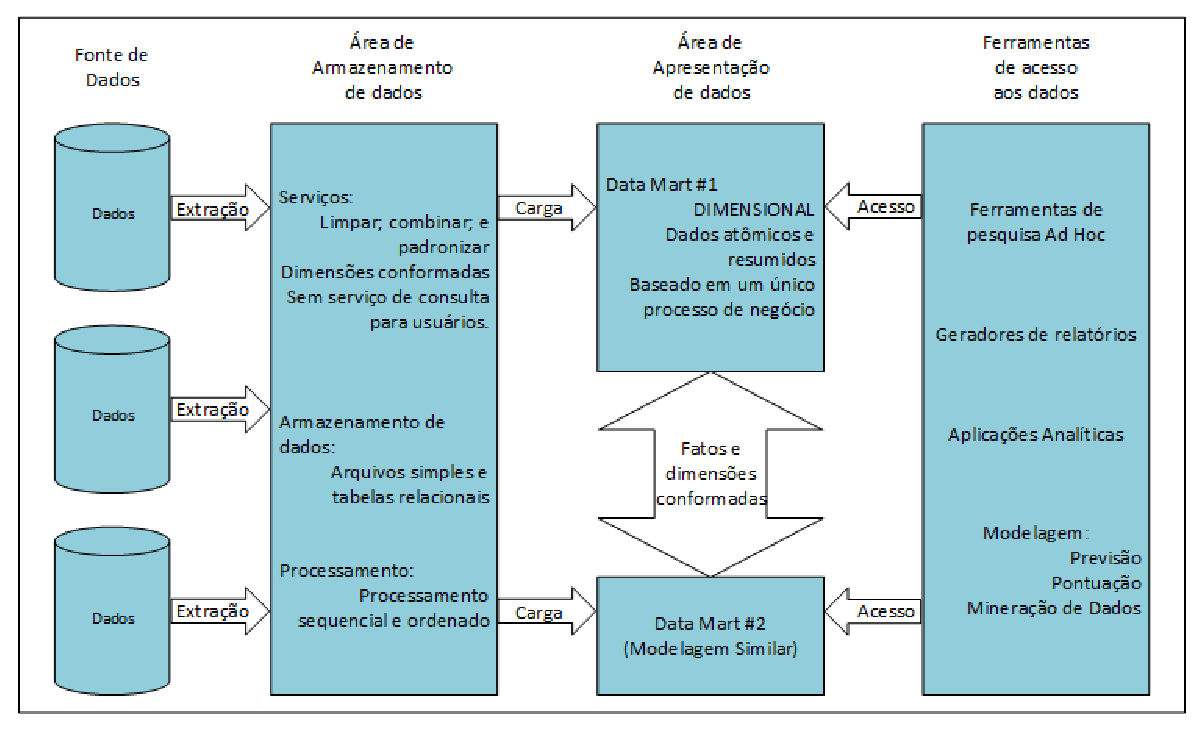
\includegraphics[scale=0.7]{figuras/componentesdw.eps}
		\caption{Componentes de um \textit{Data Warehouse}. Fonte \cite{kimball}}
		\label{componentesdw}
\end{figure}

\subsection{Operational Source Systems - OSS}
Esses são os sistemas operacionais de registro que capturam as transações do negócio, ou seja, esses sistemas operacionais são as fontes de coleta dos dados, das informações, do negócio. Portanto, são fontes que estão fora do escopo do DW, pois se tem pouco ou nenhum controle sobre o conteúdo e o formato dos dados. Por serem conhecidos como sistemas orientados a processo (OLTP, sigla em inglês), esses sistemas devem ter alto desempenho e disponibilidade. Os dados provenientes do OSS são parte da infra-estrutura da organização e são, geralmente, detalhados, atualizáveis e não-redundantes. \cite{kimball}

\subsection{Data Staging Area - DSA}
Área de armazenagem de dados é tanto uma área de armazenamento como um conjunto de processos comumente identificados como o Extração-Transformação-Carga (ETL, sigla em inglês). Essas área armazenagem é tudo que existe entre os sistemas operacionais de origem e a área de apresentação de dados. Em um \textit{\textit{Data Warehouse}} os dados operacionais brutos são transformados e ajustados para consulta do usuário e consumo dos mesmos. \cite{kimball}

\subsubsection{ETL}
Extração é o primeiro passo no processo de obtenção de dados para o ambiente do \textit{\textit{Data Warehouse}}. Uma vez que os dados são extraídos para a área de armazenamento, existem inúmeras potenciais transformações que podem ser realizadas, como por exemplo: limpeza dos dados (correção ortografia, resolver conflitos de domínio, lidar com elementos em falta, ou converter para formatos padrão ); combinação de dados de várias fontes; duplicação de dados; atribuição de chaves do DW. Transformações são precursoras para o carregamento dos dados, passo final do processo de ETL, na área de apresentação do \textit{\textit{Data Warehouse}}, e carregar dados no ambiente de \textit{\textit{Data Warehouse}} normalmente leva à forma de apresentação em tabelas dimensionais.
\cite{kimball} afirma que ETL é um processo crítico e pode consumir até 85% de todo o esforço global na criação e manutenção de um ambiente DW.

\subsection{Data Presentation}
A área de apresentação de dados é onde os dados são organizados, armazenados e disponibilizados para consulta direta pelos usuários, geradores de relatórios e outras aplicações analíticas. Essa é a área onde o stakeholder e usuários têm acesso. De modo geral, referem-se a área de apresentação de dados como uma série data marts integrados. \cite{kimball}

Um data mart é uma fatia da área total da apresentação, ou seja, minimalistamente falando, um data mart apresenta os dados de um único processo de negócio. Os data marts da área de apresentação devem contar dados atômicos e detalhados. Dados atômicos são necessários para evitar consultas imprevisíveis por conta dos usuários. \cite{kimball}

\subsection{Data Access Tools - DAT}
Ferramentas de acesso a dados nada mais é que as mais diversas formas de acesso aos dados da área de apresentação, e uma forma bem comum é através de ferramentas. Uma ferramenta de acesso a dados pode ser tão simples como uma ferramenta de consulta ad hoc ou tão complexo como uma mineração de dados sofisticado ou aplicação de modelagem. Cerca de 80 a 90 por cento do usuários serão atendidos por ferramentas que são basicamente modelos acabados que não permitem aos usuários construir consultas relacionais diretamente. \cite{kimball}

\section{Modelagem Dimensional}
Modelagem dimensional é uma técnica para modelar banco de dados e deixá-los simples e compreensíveis, contém as mesmas informações que um modelo normalizado, porém empacota os dados em um formato cujo os objetivos são a compreensão do usuário, o desempenho de queries, e a resistência à mudança. \cite{kimball}

\subsection{Tabela Fato}
Uma tabela fato é uma estrutura que contém muitas ocorrências de dados e representa os dados que ocorrem muitas vezes. É a primeira tabela em um modelo dimensional em que o as medições numérica de desempenho são armazenadas e o termo fato é utilizado para representar uma medida de negócio, onde uma medição é feita na intersecção de todas as dimensões do negócio.  A lista de dimensões define o grão da tabela de fatos e diz qual o escopo da medição. \cite{kimball}

Fatos aditivos são fatos acumulado. Acumular medições é crucial porque as aplicações de \textit{Data Warehouse} quase nunca recuperam uma única linha da tabela fato. Em vez disso, eles trazem de volta centenas, milhares, ou até milhões de linhas fato de cada vez, e o melhor a se fazer com tantas linhas é acumula-las. Como por exemplo, o total (soma) de produtos vendidos.

Fatos semi-aditivo, são fatos que apresentam um resumo de alguma medição, e esse resumo não pode ser efetuado através de uma soma, e sim através de alguma medida de posição, como por exemplo a média aritmética.

Factos não aditivos são fatos que não podem ser logicamente resumidos entre linhas, ou seja, não pode ser agrupados, como por exemplo porcentagens e proporções. Os fatos mais úteis em uma tabela de fatos são numéricos e aditivos.

As tabela fatos possuem uma das três categorias:
\begin{itemize}
	\item Transação: é a mais comum e representa um nível individual de transações, ou seja, essas tabelas representam um evento que ocorrer em um instante qualquer no tempo. Um linha na tabela fato existe a partir de cada uma das transações de dados que acontece.
	\item Snapshot Periódico: essa tabela é necessária para visualizar o desempenho cumulativo do negócio em intervalos regulares e previsíveis de tempo. Ao contrário da tabela de transação, onde a carga é realizada em uma linha por ocorrência, na de snapshot periódico, tem-se um retrato da atividade no final de um dia, semana, ou mês, e depois novamente no final do próximo período. São mais complexas do que as de transação e representação uma agregação de atividades de transação que ocorreram durante um período de tempo.
	\item Snapshot Acumulado: essa tabela é representada por acumular transações em períodos de tempo indeterminado, podendo abranger a vida completa de uma transação ou produto.

\end{itemize}
Tabelas fato tem duas ou mais chaves estrangeiras que se conectam a chaves primárias das tabelas de dimensão. Quando todas as chaves na tabela fato correspondem à respectiva chave primária corretamente na tabela dimensão correspondente, se diz que as tabelas satisfazem a propriedade de integridade referencial.

Cada tabela fato tem sua própria chave primária composta por um subconjunto de chaves estrangeiras, que é conhecida como chave composta ou concatenada. Toda tabela fato em um modelo dimensional tem uma chave composta e, inversamente, toda tabela que tem uma chave composta é uma tabela fato. E outra maneira de identificar é que toda tabela que expressa um relacionamento de muitos-para-muitos é uma tabela fato.

\subsection{Tabelas Dimensão}
As tabelas dimensão contém as descrições textuais do negócio. Em um modelo dimensional bem projetado, tabelas de dimensão tem muitas colunas ou atributos. Estes atributos descrevem as linhas na tabela de dimensão. Não é incomum uma tabela dimensão ter de 50 a 100 atributos. As tabelas de dimensões tendem a ser relativamente pequenas em termos de número de linhas, mas são enormes em largura com várias colunas. Cada dimensão é definida pela sua chave primária, que serve como base para a integridade referencial com qualquer tabela fato que ela esteja associada.

Atributos de dimensão servem como a fonte principal de restrições de consulta, agrupamentos e relatórios. Em uma consulta(query) ou solicitação de relatório, os atributos são identificados pela palavra POR. Por exemplo, total vendido POR semana. O poder do \textit{Data Warehouse} é diretamente proporcional à qualidade e profundidade dos atributos de dimensão.

\section{Processo de Modelagem Dimensional}
\begin{enumerate}
	\item Processo de Negócio
Selecione o processo de negócio a modelar.
Um processo é uma atividade natural realizada na organização que normalmente é apoiado por uma fonte de coleta de dados. É preciso garantir a consistência dos dados efetuando uma única operação de carga, por exemplo.
	\item Grain 
Declare o grão do processo de negócio.
Declarar o grão significa especificar exatamente o que uma linha da tabela de fato representa. O grão transmite o nível de detalhe associado com as medidas da tabela fatos. Ele fornece a resposta para a pergunta: "Como você descreveria uma única linha na tabela fato?"
	\item Dimensões 
Escolha as dimensões que se aplicam a cada linha da tabela fato.
Com a escolha de cada dimensão, lista-se atributos que irão detalhar cada tabela de dimensão.
	\item Fatos 
Identifique os fatos numéricos que irão preencher cada linha da tabela fato.
Os fatos são determinado pela resposta à pergunta: "O que estamos medindo?"
Os stakeholders estão muito interessados em analisar a medida de desempenho de cada um dos processos de negócio.
\end{enumerate}

\subsection{Tipos de Schema}
Segundo KIMBALL (2002) existem três esquemas para modelagem multidimensional:

\subsubsection{Esquema estrela}
É o esquema mais popular em \textit{Data Warehouse}, por que oferece um desempenho melhor das consultas (queries) a serem executadas, especialmente em consultas grandes se comparado com o modelo relacional e além disso tem a grande vantagem de ser mais fácil de entender.
Consiste de uma tabela fato circundada (ligada por relações) por um conjunto de tabelas dimensão. Quando desenhando, assemelha-se a forma de uma estrela, daí o nome. As tabelas de dimensões não são desnormalizada. \cite{redbooks}

\subsubsection{Esquema Floco de Neve}
Normalizando e expandindo o tamanho das tabelas dimensão no esquema estrela resultará na implementação do esquema floco de neve. A dimensão é dita floco de neve quando as colunas de baixa cardinalidade da dimensão são separadas em tabelas normalizadas que então se relacionam de volta para a tabela dimensão de origem. \cite{redbooks}

\subsubsection{Esquema Constelação de Fatos}
O Esquema Constelação de Fatos é constituído de duas ou mais tabelas fatos unidas por uma ou mais dimensões. Esse tipo de esquema pode ser visto como uma coleção de esquemas estrela. \cite{redbooks} Para \textit{Data Warehouse}s, o esquema de Constelação de Fatos é mais comumente utilizado, visto que ele pode modelar assuntos múltiplos e inter-relacionados. \cite{gouveia2009}

A figura \ref{tresesquemas} ilustra os três esquemas acima citados.

\begin{figure}[!htb]
	\centering
		
\includegraphics{figuras/tresesquemas.eps}
		\caption{(a)Esquema Estrela. (b) Esquema Floco de Neve. (c) Esquema Constelação de Fatos. Fonte \cite{redbooks}}
		\label{tresesquemas}
\end{figure}

\subsection{Arquitetura}
O DW pode ter um estrutura centralizada ou distribuída em camadas que são conhecidas como: (1) repositório; (2) apresentação, e (3) ETL. camada ETL é a responsável por capturar dados de várias fontes heterogeneas, transformas, integrar e carrega-los no DW consolidado. A camada de repositório representa o próprio DW, e a camada de apresentação fornece funcionalidades analiticas para acessar o DW.

\begin{figure}[!htb]
	\centering
		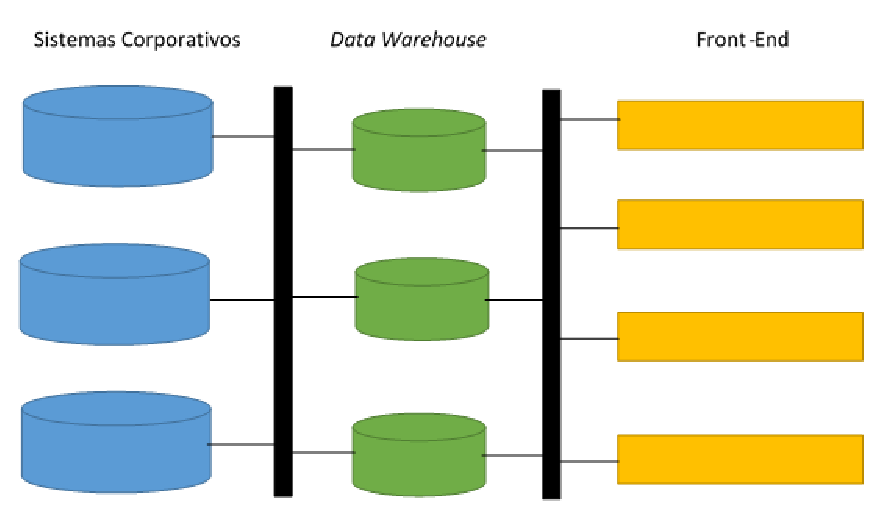
\includegraphics[scale=0.7]{figuras/arqemcamadas.eps}
		\caption{Arquitetura em camadas. Fonte \cite{kimball}}
		\label{arqemcamadas}
\end{figure}

No modelo centralizado de um DW, o poder de processamento é maior e os processos de busca de informação podem ser otimizados. A arquitetura em camadas é mais flexível e permite consultas simultâneas sem muita perda de performance. Na primeira camada é disponibilizado o servidor que atende a maior parte das consultas, com baixo volume de dados. Nas demais camadas tem-se os servidores com volume maior de dados que atenderão a uma quantidade menor de usuários. \cite{kimball}

\begin{figure}[!htb]
	\centering
		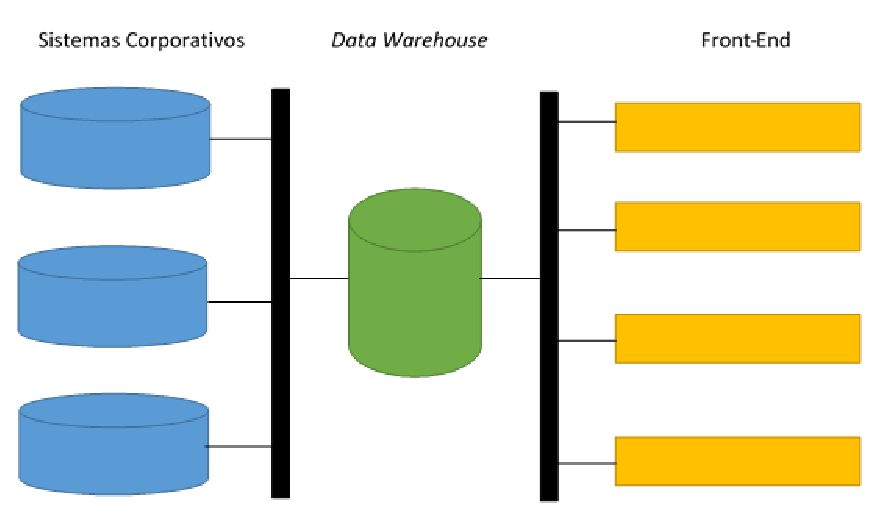
\includegraphics[scale=0.7]{figuras/arqcentralizada.eps}
		\caption{Arquitetura centralizada. Fonte \cite{redbooks}}
		\label{arqcentralizada}
\end{figure}

\section{OLAP}

Sistemas de \textit{Data Warehouse} servem para os usuários como uma ferramenta de análise de dados e tomada de decisão, muito diferente dos sistemas de banco de dados operacionais, que tem a característica de executarem transações \textit{on-line} (OLTP, sigla em inglês). Os sistemas de \textit{Data Warehouse} podem organizar e apresentar os dados em vários formatos com o intuito de satisfazer as necessidades de diferentes usuário, para isso, executa-se o processamento analítico \textit{on-line} (OLAP, em inglês). \cite{han}

Um sistema OLAP tem por características: 
\begin{itemize}
	\item Gerencia enormes quantidades de dados históricos, fornecendo facilidades de agregação de dados, e armazenando informações em diferentes níveis de granularidade. \cite{han}
	\item É modelado por assunto e representado pelos esquemas estrela, floco de neve e constelação de fatos. \cite{han}
	\item Abrange, muitas vezes, diversas versões de esquema de banco de dados, de acordo com a evolução dos processos da organização, e também lida com informações de diferentes fontes de origem, integrando-as e agregando valor ao negócio. \cite{han}
	\item Permite acesso apenas de leitura, apesar de algumas consultas serem extremamente complexas. \cite{han}
\end{itemize}

Toda a definição e execução de operações OLAP se baseiam no modelo multidimensional de dados que permite visualizar os dados gerados em forma de um cubo, ou seja, é possível modelar e visualizar os dados nas dimensões de um cubo. Todo modelo multidimensional é organizado em torno de um tema central, que no contexto de \textit{DW}, é representado por uma tabela fato identificadas na modelagem, e as tabelas dimensão são representadas pelas dimensões do cubo, que podem ter três dimensões, quatro dimensões, n-dimensões. \cite{han}
A figura abaixo ilutra um cubo 3-D.

\begin{figure}[!htb]
	\centering
		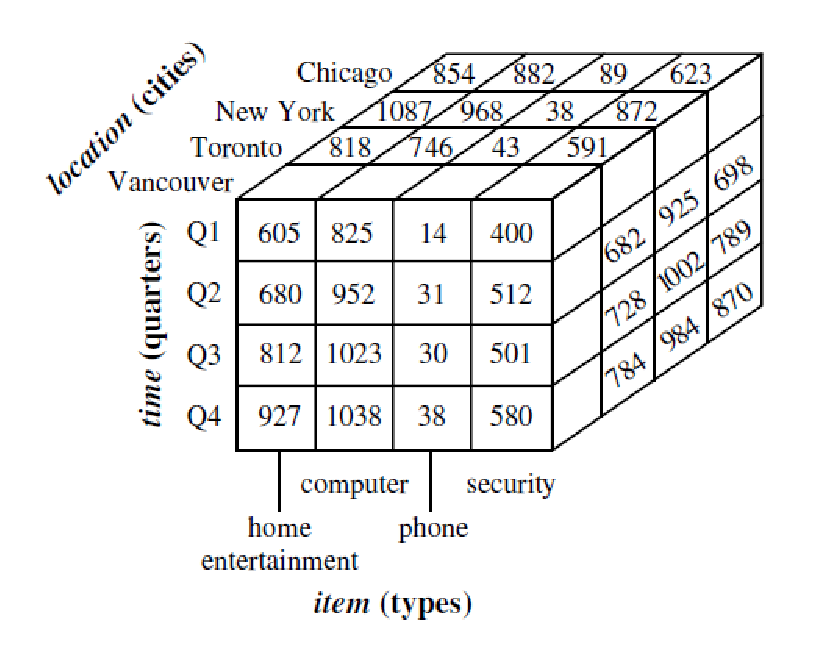
\includegraphics{figuras/cubo3d.eps}
		\caption{Cubo 3-D. Fonte \cite{han}}
		\label{arqcentralizada}
\end{figure}

A análise multidimensional tem se tornado um caminho popular para estender a capacidade de consultas queries e de geração de relatórios, isto é, a análise multidimensional, ao invés de realizar várias consultas em um banco de dados, ela estrutura os dados permitindo um acesso rápido e fácil às respostas das perguntas dos usuários. Esse acesso facilitado e rápido é permitido através de pré cálculos realizados com antecedência e tornando as respostas prontamente disponíveis, ou seja, como as consultas já estão realizadas, já se sabe o resultado de cada uma, então o retorno da consulta é praticamente instantâneo. \cite{redbooks}

Em um modelo multidimensional, os dados são organizados em diversas dimensões, e cada dimensão contém múltiplos níveis de abstração definidos pelo conceito de hierarquias. Esta organização permite aos usuários flexibilidade para visualizar os dados a partir de perspectivas diferentes e em relações complexas\cite{han}, oferecendo aos usuários a possibilidade de olhar para um números enorme de fatores interdependentes envolvidos em um problema de negócio. \cite{redbooks}

Existem algumas operações OLAP executáveis em cubo que materializam esses diferentes pontos de vista, permitindo a consulta (\textit{query}) interativa e a análise dos dados na mão. Dessa maneira, as operações OLAP oferecem um ambiente amigável para análise interativa de dados. \cite{han}

As operações mais conhecidas são:
\begin{itemize}
	\item \textit{Roll-up}: também chamada de \textit{drill-up}, executa agregação em um cubo de dados, podendo ser subindo uma hierarquia de conceitos para uma dimensão ou reduzindo a dimensão. Quando a operação \textit{Roll-up} é realizada por redução de dimensão, uma ou mais dimensões são removidas do cubo. \cite{han}
	\item \textit{Drill-down}: a operação \textit{Drill-down} é o inverso da operação \textit{Roll-up}. Ela navega a partir de dados menos detalhados para dados mais detalhados. Essa operação pode ser realizada descendo uma hierarquia de conceitos para uma dimensão ou introduzindo outras dimensões. \cite{han}
	\item \textit{Slice and dice}: A operação \textit{Slice and dice} realiza uma seleção em uma dimensão do cubo, resultando em um subcubo. \cite{han}
	
		Define um membro ou um grupo de membros que estão separados, de todas as outras dimensões, e depois realiza o cruzamento com essas dimensões. Por exemplo, as dimensões produto, lojas e tempo, ao isolar dois atributos de produto (leite e biscoito), ao se desejar saber o total de leites e biscoitos vendidos por todas as loja, realiza-se então uma operação \textit{Slice}.
		
		A operação \textit{dice} seria então juntar membros de uma dimensão em um cubo com os outros diversos membros das outras dimensões, seguindo o exemplo anterior, o cubo seria montado por datas e por lojas especificas.
	\item \textit{Pivot}: também chamado de \textit{rotate} é uma operação de visualização que rotacional o eixo em vista de modo a proporcionar uma apresentação alternativa dos dados, ou seja, realiza uma troca de dimensões, colunas. \cite{han}\cite{redbooks}
\end{itemize}

Enquanto os tradicionais mecanismos OLAP e de geração de relatórios são valiosos para a análise de tendências passadas, os mecanismos de monitoramento e previsão são necessários para melhorar o conhecimento do desempenho atual, bem como para a previsibilidade e a detecção precoce de um comportamento inesperado. \cite{spdw}

Um ambiente DW contribui para a representação de métricas, sejam elas de produto, processo ou projeto, em um modelo multidimensional, e contribui também para diminuir a intromissão nos processos de ETL, no apoio às atividades de monitoramento que possuem uma frequente e grande quantidade de carga de dados, consistência e confiabilidade dos dados, entre outros. \cite{spdw}

A intrusão pode ser interpretada como um nível de envolvimento de recursos e humanos durante a execução do processo de captura de dados e \apudonline{spdw}{gopal} afirmam que intrusão é um dos fatores cruciais de aceitação de um plano de métricas.

Apoiado nas premissas:
\begin{itemize}
	\item Mecanismos OLAP e de geração de relatórios;
	\item Mecanismos de monitoramento e previsão;
	\item Representação de métricas em um modelo multidimensional; e,
	\item Diminuição de intromissão;
\end{itemize}

É que esse projeto de Trabalho de Conclusão de Curso firma seu alicerce para fornecer um arcabouço de ferramentas que ofereça essas premissas reunidas em um só ambiente.

